% T402 Multi-Chain Support - Standalone TikZ
% Compile with: pdflatex multichain.tex

\documentclass[tikz,border=10pt]{standalone}
\usepackage{tikz}
\usetikzlibrary{arrows.meta, shapes.geometric, positioning, calc, fit}
\usepackage{xcolor}

% Define colors
\definecolor{t402blue}{HTML}{3B82F6}
\definecolor{t402green}{HTML}{10B981}
\definecolor{t402purple}{HTML}{8B5CF6}
\definecolor{t402gray}{HTML}{6B7280}
\definecolor{ethblue}{HTML}{627EEA}
\definecolor{solpurple}{HTML}{9945FF}
\definecolor{tonblue}{HTML}{0098EA}
\definecolor{tronred}{HTML}{FF0013}

\begin{document}
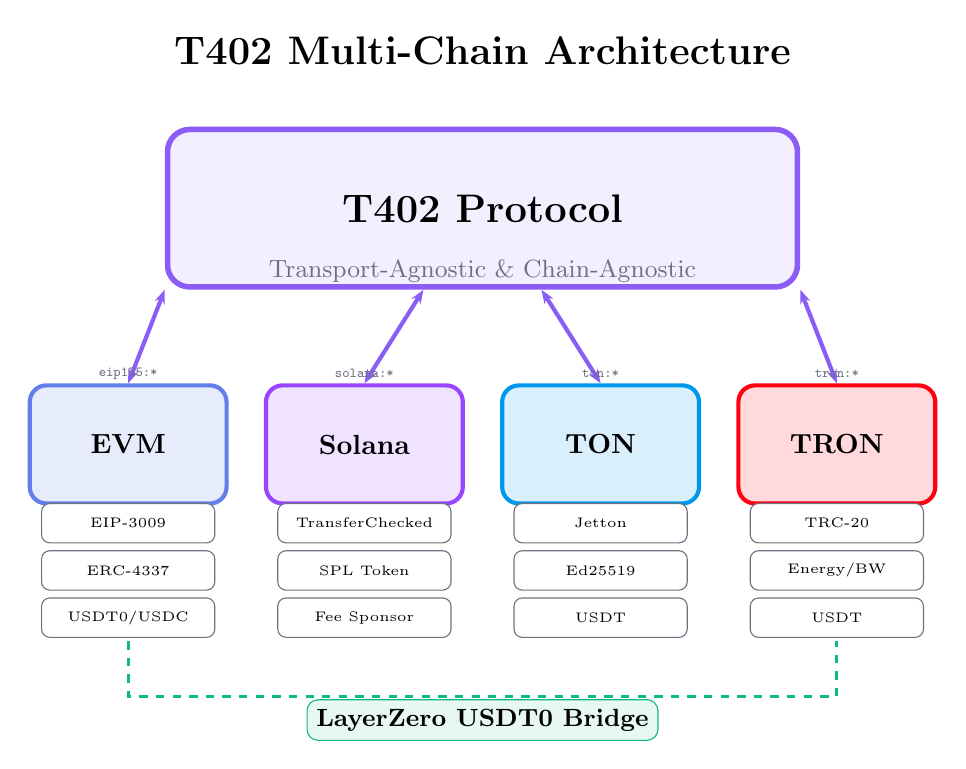
\begin{tikzpicture}[
    chain/.style={
        rectangle,
        rounded corners=6pt,
        minimum width=2.5cm,
        minimum height=1.5cm,
        draw=#1,
        line width=1.5pt,
        fill=#1!15,
        font=\bfseries
    },
    protocol/.style={
        rectangle,
        rounded corners=8pt,
        minimum width=8cm,
        minimum height=2cm,
        draw=t402purple,
        line width=2pt,
        fill=t402purple!10,
        font=\bfseries\Large
    },
    feature/.style={
        rectangle,
        rounded corners=3pt,
        minimum width=2.2cm,
        minimum height=0.5cm,
        draw=t402gray,
        fill=white,
        font=\tiny
    },
    arrow/.style={
        <->,
        >={Stealth[length=5pt]},
        line width=1.5pt,
        t402purple
    }
]

% Title
\node[font=\bfseries\Large] at (0,5) {T402 Multi-Chain Architecture};

% Protocol layer
\node[protocol] (t402) at (0,3) {T402 Protocol};

% Subtitle
\node[font=\small, t402gray] at (0,2.2) {Transport-Agnostic \& Chain-Agnostic};

% Chains
\node[chain=ethblue] (evm) at (-4.5,0) {EVM};
\node[chain=solpurple] (sol) at (-1.5,0) {Solana};
\node[chain=tonblue] (ton) at (1.5,0) {TON};
\node[chain=tronred] (tron) at (4.5,0) {TRON};

% Features under each chain
\node[feature] at (-4.5,-1) {EIP-3009};
\node[feature] at (-4.5,-1.6) {ERC-4337};
\node[feature] at (-4.5,-2.2) {USDT0/USDC};

\node[feature] at (-1.5,-1) {TransferChecked};
\node[feature] at (-1.5,-1.6) {SPL Token};
\node[feature] at (-1.5,-2.2) {Fee Sponsor};

\node[feature] at (1.5,-1) {Jetton};
\node[feature] at (1.5,-1.6) {Ed25519};
\node[feature] at (1.5,-2.2) {USDT};

\node[feature] at (4.5,-1) {TRC-20};
\node[feature] at (4.5,-1.6) {Energy/BW};
\node[feature] at (4.5,-2.2) {USDT};

% Connections
\draw[arrow] (t402.south west) -- (evm.north);
\draw[arrow] (t402.south) ++(-0.75,0) -- (sol.north);
\draw[arrow] (t402.south) ++(0.75,0) -- (ton.north);
\draw[arrow] (t402.south east) -- (tron.north);

% Chain IDs
\node[font=\tiny\ttfamily, t402gray] at (-4.5,0.9) {eip155:*};
\node[font=\tiny\ttfamily, t402gray] at (-1.5,0.9) {solana:*};
\node[font=\tiny\ttfamily, t402gray] at (1.5,0.9) {ton:*};
\node[font=\tiny\ttfamily, t402gray] at (4.5,0.9) {tron:*};

% LayerZero bridge
\node[rectangle, rounded corners=4pt, draw=t402green, fill=t402green!10, font=\small\bfseries] at (0,-3.5) {LayerZero USDT0 Bridge};
\draw[t402green, dashed, line width=1pt] (-4.5,-2.5) -- (-4.5,-3.2) -- (4.5,-3.2) -- (4.5,-2.5);

\end{tikzpicture}
\end{document}
